\paragraph{$\Lambda$ Reconstruction}
\label{LambdaReconstruction}

The following cuts were used to select good $\Lambda$ ($\bar{\Lambda}$) candidates:

\begin{enumerate}
 \item{Cuts Common to Both Daughters}
 \begin{enumerate}
  \item $|\eta| < 0.8$
  \item SetTPCnclsDaughters(80)
  \item SetStatusDaughters(AliESDtrack::kTPCrefic)
  \item SetMaxDcaV0Daughters(0.4)
 \end{enumerate}


 \item Pion Specific Daughter Cuts
 \begin{enumerate}
  \item $p_{T} > 0.16$
  \item DCA to prim vertex $>$ 0.3
 \end{enumerate} 
 
 \item Proton Specific Daughter Cuts
  \begin{enumerate}
  \item $p_{T} > $
  \begin{itemize}
   \item 0.5 ($p$)
   \item 0.3 ($\bar{p}$)
  \end{itemize}
   \item DCA to prim vertex $>$ 0.1 
 \end{enumerate} 
 
 \item Lambda Cuts
 \begin{enumerate}
  \item $|\eta| < 0.8$
  \item $p_{T} > 0.4$
  \item $|m_{inv} - m_{PDG}| <$ 3.8 MeV
  \item Cosine of pointing angle $>$ 0.9993
  \item OnFlyStatus = false
  \item Decay Length $<$ 60 cm
 \end{enumerate}  
 
\end{enumerate}

\begin{figure}
  \centering
  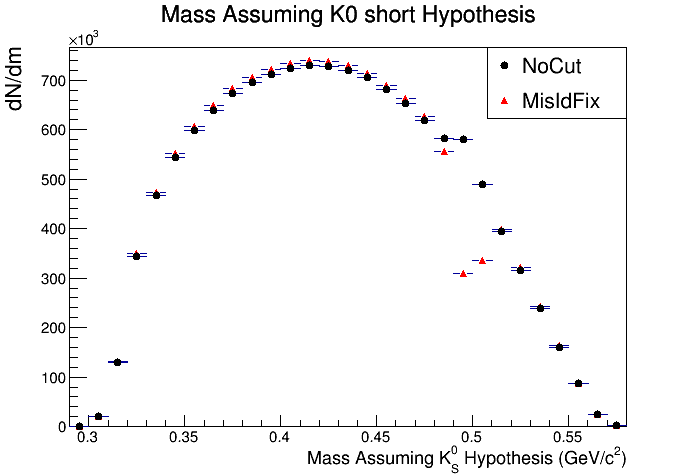
\includegraphics[width=100mm]{3_DataSelection/Figures/MassAssumingK0ShortHypothesis.png}
  \caption{Here is a caption}
  \label{fig:MassAssK0ShortHyp}
\end{figure}